% Proceedings-to-EEE pipeline for the public README.
% The visual system follows the shipped AISI Auto-BenchmarkCards figure:
% one horizontal spine, black pictograms, Blue700 transport arrows, numbered
% stage labels below, and a concrete output artifact at the right.
\documentclass[tikz,border=3pt]{standalone}

\usepackage{newtxtext,newtxmath}
\usepackage{xcolor}
\usepackage{tikz}
\usetikzlibrary{arrows.meta,calc}

\definecolor{Ink}{HTML}{1A1A1A}
\definecolor{Ink60}{HTML}{6E6E6E}
\definecolor{Rule}{HTML}{D9D9D9}
\definecolor{Blue700}{HTML}{1F4E9C}
\definecolor{Carmine}{HTML}{B2182B}

% Frozen paper, supplement, and repository sources.
\newcommand{\icnFreeze}[2]{%
\begin{scope}[shift={#1}]
\begin{scope}[x={#2},y={#2},shift={(0.35,0.12)},line join=round,line cap=butt]
  \foreach \ang in {13,6}{%
    \begin{scope}[rotate around={\ang:(-3.4,-4.0)}]
      \fill[white] (-3.4,-4.0) rectangle (2.2,3.0);
      \draw[Ink,line width=1.05pt,rounded corners=0.5mm]
            (-3.4,-4.0) rectangle (2.2,3.0);
    \end{scope}}
  \fill[Ink,rounded corners=0.5mm] (-3.4,-4.0) rectangle (2.2,3.0);
  \fill[white] (-2.65,1.25) rectangle (1.45,2.15);
  \foreach \yy in {0.15,-1.05}{
    \draw[white,line width=0.82pt] (-2.65,\yy)--(1.45,\yy);}
  \draw[white,line width=0.82pt] (-2.65,-2.25)--(-0.55,-2.25);
  % Small lock marks that the bytes and manifest are fixed.
  \fill[white,rounded corners=0.35mm] (0.15,-3.45) rectangle (2.75,-1.15);
  \draw[Ink,line width=0.95pt,rounded corners=0.35mm]
        (0.15,-3.45) rectangle (2.75,-1.15);
  \draw[Ink,line width=0.95pt] (0.70,-1.15) arc (180:0:0.75 and 0.90);
  \fill[Ink] (1.45,-2.32) circle (0.22);
\end{scope}\end{scope}}

% Page layout, result blocks, and the dense-row proposal channel.
\newcommand{\icnDiscover}[2]{%
\begin{scope}[shift={#1}]
\begin{scope}[x={#2},y={#2},shift={(-0.15,0.05)},line join=round,line cap=butt]
  \draw[Ink,line width=1.05pt,rounded corners=0.55mm,fill=white]
        (-5.2,-4.6) rectangle (1.8,4.2);
  \fill[Ink] (-4.25,2.65) rectangle (0.80,3.35);
  \fill[Ink60] (-4.25,1.25) rectangle (-0.65,1.95);
  \fill[Blue700] (-4.25,-0.20) rectangle (0.80,0.72);
  \fill[Blue700] (-4.25,-1.65) rectangle (0.15,-0.73);
  \foreach \xx in {-2.55,-0.80}{
    \draw[white,line width=0.50pt] (\xx,-1.65)--(\xx,0.72);}
  \draw[white,line width=0.50pt] (-4.25,-0.73)--(0.80,-0.73);
  \draw[Ink60,line width=0.65pt,dash pattern=on 1.2pt off 0.9pt]
        (-4.55,-2.55)--(1.10,-2.55);
  % Candidate slips emerging from the discovered regions.
  \foreach \yy in {1.55,0,-1.55}{%
    \draw[Ink,line width=0.85pt,rounded corners=0.45mm,fill=white]
      (2.75,\yy-0.62) rectangle (5.35,\yy+0.62);
    \draw[Blue700,line width=0.85pt] (3.20,\yy+0.20)--(4.85,\yy+0.20);
    \draw[Ink60,line width=0.60pt] (3.20,\yy-0.20)--(4.45,\yy-0.20);}
  \draw[Ink,line width=0.75pt,-{Stealth[length=2.0mm,width=1.5mm]}]
        (1.95,0)--(2.55,0);
\end{scope}\end{scope}}

% Candidate evidence is narrowed to verified support, semantics, cell identity,
% and producer origin. Ambiguity remains outside canonical composition.
\newcommand{\icnResolve}[2]{%
\begin{scope}[shift={#1}]
\begin{scope}[x={#2},y={#2},shift={(-0.35,0.30)},line join=round,line cap=butt]
  \foreach \xx in {-2.8,0,2.8}{
    \fill[Ink,rounded corners=0.30mm] (\xx-1.10,3.45) rectangle (\xx+1.10,4.55);}
  \fill[Ink,even odd rule]
        (-5.0,2.75)--(5.0,2.75)--(1.05,-1.15)--(1.05,-2.20)--
        (-1.05,-2.20)--(-1.05,-1.15)--cycle
        (-3.25,1.70)--(3.25,1.70)--(0.33,-1.38)--(0.33,-2.20)--
        (-0.33,-2.20)--(-0.33,-1.38)--cycle;
  \fill[Ink,rounded corners=0.50mm] (-2.85,-5.10) rectangle (2.85,-2.65);
  \foreach \yy in {-3.35,-4.10}{
    \draw[white,line width=0.82pt] (-2.00,\yy)--(2.00,\yy);}
  \draw[white,line width=0.82pt] (-2.00,-4.78)--(0.20,-4.78);
  \draw[white,line width=1.05pt] (-0.70,-3.72)--(-0.10,-4.28)--(1.02,-3.05);
\end{scope}\end{scope}}

% Positive producer origin and all export predicates precede deterministic JSON
% composition. Ineligible candidates remain in the review layer drawn at right.
\newcommand{\icnCompose}[2]{%
\begin{scope}[shift={#1}]
\begin{scope}[x={#2},y={#2},shift={(0,0.10)},line join=round,line cap=round]
  \fill[Ink] (-4.45,0)--(-1.80,2.65)--(0.85,0)--(-1.80,-2.65)--cycle;
  \draw[white,line width=1.10pt] (-3.00,0.05)--(-2.15,-0.78)--(-0.48,1.05);
  \draw[Ink,line width=0.95pt,-{Stealth[length=2.0mm,width=1.55mm]}]
        (1.02,0)--(1.48,0);
  \fill[Ink,rounded corners=0.45mm] (1.65,-3.05) rectangle (5.20,3.05);
  \fill[white] (3.72,3.05)--(5.20,1.57)--(3.72,1.57)--cycle;
  \foreach \yy/\xe in {0.85/4.45,-0.20/3.88,-1.25/4.45}{
    \draw[white,line width=0.82pt] (2.28,\yy)--(\xe,\yy);}
  \draw[white,line width=0.82pt] (2.28,-2.20)--(3.25,-2.20);
\end{scope}\end{scope}}

% Chunky transport arrow from the shipped AISI figure geometry.
\newcommand{\barrow}[2]{%
  \filldraw[fill=Blue700,draw=Blue700,line width=1.0pt,line join=round]
    (#1,#2+0.168) -- (#1+0.483,#2+0.168) -- (#1+0.483,#2+0.337)
    -- (#1+0.820,#2) -- (#1+0.483,#2-0.337) -- (#1+0.483,#2-0.168)
    -- (#1,#2-0.168) -- cycle;}

\begin{document}
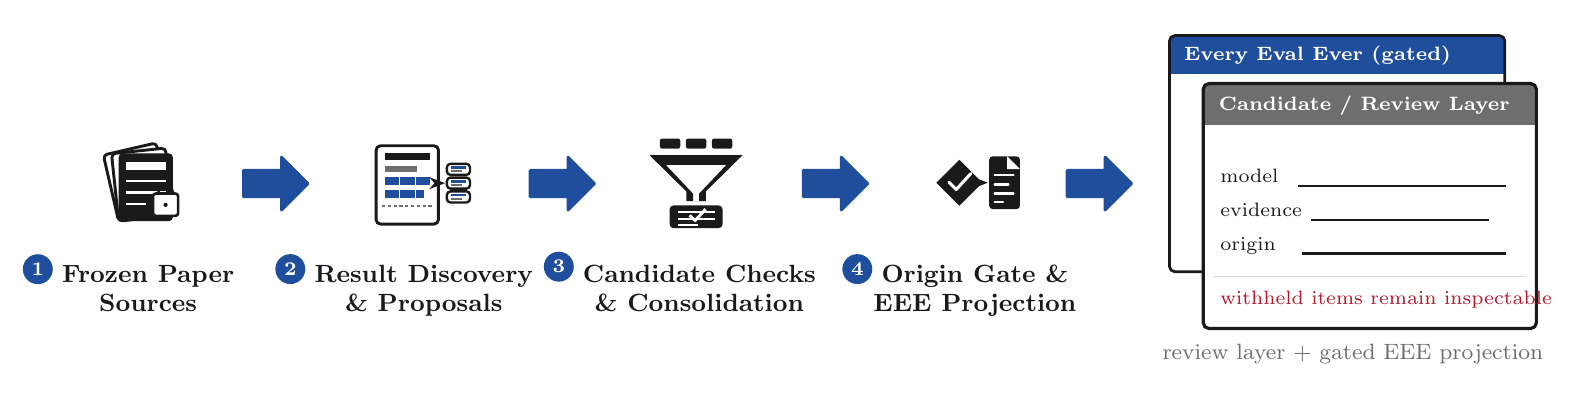
\begin{tikzpicture}[
  x=1cm,y=1cm,line join=round,line cap=butt,font=\scriptsize,
  ttl/.style={font=\small\bfseries,color=Ink,anchor=base,inner sep=0pt},
  lbl/.style={font=\scriptsize,color=Ink,anchor=base west,inner sep=0pt},
  sec/.style={font=\footnotesize,color=Ink60,anchor=base,inner sep=0pt},
  badge/.style={circle,fill=Blue700,text=white,inner sep=0pt,
                minimum size=3.8mm,font=\scriptsize\bfseries}
]
\path[use as bounding box] (-0.18,1.28) rectangle (19.24,-3.22);

% Four-stage AISI spine.
\icnFreeze{(1.35,-0.70)}{1.23mm}
\icnDiscover{(4.85,-0.70)}{1.13mm}
\icnResolve{(8.35,-0.70)}{1.18mm}
\icnCompose{(11.85,-0.70)}{1.10mm}
\barrow{2.56}{-0.70}
\barrow{6.20}{-0.70}
\barrow{9.67}{-0.70}
\barrow{13.02}{-0.70}

% Stage names.
\node[ttl] (t1) at (1.35,-1.95) {Frozen Paper};
\node[badge] at ($(t1.west)+(-0.30,0.085)$) {1};
\node[ttl] at (1.35,-2.32) {Sources};

\node[ttl] (t2) at (4.85,-1.95) {Result Discovery};
\node[badge] at ($(t2.west)+(-0.30,0.085)$) {2};
\node[ttl] at (4.85,-2.32) {\& Proposals};

\node[ttl] (t3) at (8.35,-1.95) {Candidate Checks};
\node[badge] at ($(t3.west)+(-0.30,0.085)$) {3};
\node[ttl] at (8.35,-2.32) {\& Consolidation};

\node[ttl] (t4) at (11.85,-1.95) {Origin Gate \&};
\node[badge] at ($(t4.west)+(-0.30,0.085)$) {4};
\node[ttl] at (11.85,-2.32) {EEE Projection};

% Conditional EEE projection behind the always-preserved candidate/review layer.
\fill[white,rounded corners=2pt] (14.32,-1.82) rectangle (18.58,1.18);
\begin{scope}
  \clip[rounded corners=2pt] (14.32,-1.82) rectangle (18.58,1.18);
  \fill[Blue700] (14.32,0.69) rectangle (18.58,1.18);
\end{scope}
\draw[rounded corners=2pt,draw=Ink,line width=1.0pt]
      (14.32,-1.82) rectangle (18.58,1.18);
\node[font=\scriptsize\bfseries,text=white,anchor=base west,inner sep=0pt]
      at (14.50,0.86) {Every Eval Ever (gated)};

% Candidate/review layer in front. This is produced even when no candidate passes
% the positive-origin and export gates.
\begin{scope}
  \clip[rounded corners=2pt] (14.75,-2.54) rectangle (18.98,0.57);
  \fill[white] (14.75,-2.54) rectangle (18.98,0.57);
  \fill[Ink60] (14.75,0.05) rectangle (18.98,0.57);
\end{scope}
\draw[rounded corners=2pt,draw=Ink,line width=1.15pt]
      (14.75,-2.54) rectangle (18.98,0.57);
\node[font=\scriptsize\bfseries,text=white,anchor=base west,inner sep=0pt]
      at (14.94,0.23) {Candidate / Review Layer};
\node[lbl] at (14.96,-0.69) {model};
\draw[Ink,line width=0.85pt] (15.95,-0.73)--(18.60,-0.73);
\node[lbl] at (14.96,-1.12) {evidence};
\draw[Ink,line width=0.85pt] (16.12,-1.16)--(18.38,-1.16);
\node[lbl] at (14.96,-1.55) {origin};
\draw[Ink,line width=0.85pt] (16.00,-1.59)--(18.60,-1.59);
\draw[Rule,line width=0.45pt] (14.88,-1.88)--(18.85,-1.88);
\node[font=\scriptsize,color=Carmine,anchor=base west,inner sep=0pt]
      at (14.96,-2.23) {withheld items remain inspectable};

\node[sec] at (16.65,-2.93) {review layer + gated EEE projection};
\end{tikzpicture}
\end{document}
